% Drawing 74/04-11 -- folder 74, batch 04, archive page 78 (PDF page 79).
% Transcription: deux fibres $I_\alpha$, $I_\beta$ de deux points chacune, au-dessus de $\Lambda$.
% Kind: two fibres of two points over Lambda. Method 2 (schematic redraw from the facsimile). Status: ok.
% Notes: Two ovals I_alpha and I_beta of two points each, an arrow down to Lambda, drawn as an oval with two points.
% Coordinates: 1 unit = 1 mm = 1/100 of the crop width (bbox in page fractions: [0.08, 0.39, 0.3, 0.49]).
% Redrawn by Claude (claude-opus-5-5), issue #73, 2026-11-07; not checked by a human; not compiled (no TeX in the session).
% Rights: reproduces part of the work -- behind RENDER_TRANSCRIPTS, never published by itself.
\documentclass[tikz,border=3pt]{standalone}
\usepackage{amsmath,amssymb}
\usetikzlibrary{patterns,arrows.meta}
\tikzset{pencil/.style={black!45}, struck/.style={black!35}, mark/.style={circle,draw,inner sep=1.3pt}, pt/.style={circle,fill,inner sep=0.9pt}, opt/.style={circle,draw,fill=white,inner sep=1.1pt}}
\begin{document}
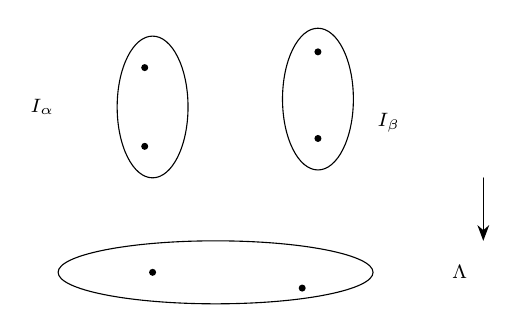
\begin{tikzpicture}[x=1mm,y=1mm,line cap=round,line join=round,font=\scriptsize]
\draw (36,-20) ellipse[x radius=4.5, y radius=9];
\draw (57,-19) ellipse[x radius=4.5, y radius=9];
\node[pt] at (35,-15) {};
\node[pt] at (35,-25) {};
\node[pt] at (57,-13) {};
\node[pt] at (57,-24) {};
\node[inner sep=1pt] at (22,-20) {\scriptsize $I_\alpha$};
\node[inner sep=1pt] at (66,-22) {\scriptsize $I_\beta$};
\draw (44,-41) ellipse[x radius=20, y radius=4];
\node[pt] at (36,-41) {};
\node[pt] at (55,-43) {};
\draw[-{Stealth[length=2mm]}] (78,-29) -- (78,-37);
\node[inner sep=1pt] at (75,-41) {\scriptsize $\Lambda$};
\end{tikzpicture}
\end{document}
